%%%%%%%%%%%%%%%%%%%%%%%%%%%%%%%%%%%%%%%%%%%%%%%%%%%%%%%%%%%%%%%%%%%%%%%%%%%%%%%
% Chapter 2: Título del capítulo 2
%%%%%%%%%%%%%%%%%%%%%%%%%%%%%%%%%%%%%%%%%%%%%%%%%%%%%%%%%%%%%%%%%%%%%%%%%%%%%%%

Siguiendo el curso del campus de la biblioteca, haciendo uso de .Q, una herramienta de búsqueda de información de la Universidad de La Laguna, se realizó una búsqueda de artículos relacionados con el Pensamiento Computacional, algunos de ellos de la famosa revista ACM.

%++++++++++++++++++++++++++++++++++++++++++++++++++++++++++++++++++++++++++++++

\section{Estado del arte}
\label{2:sec:1}

Para explicar los antecedentes y el estado actual del tema en este proyecto se tendrán en cuenta las referencias citadas a continuación:

\begin{itemize}
  \item En un artículo\cite{Tumlin:2017:TCC:3017680.3022467} publicado en 2017, \textit{"Teacher Configurable Coding Challenges for Block Languages"}, se explica como una herramienta llamada \textbf{COPPER} (CustOmizable Puzzle Programming EnviRonment), desarrollada para crear puzzles de código en una cuadrícula usando lenguajes de programación basado en bloques, 
  similar a los realizados en la plataforma Code.org "Hour of Code", tiene el potencial de incrementar el interés y el compromiso con el pensamiento computacional. 
  
  De esta manera, se fomenta la forma de pensar computacionalmente a través de tareas que mejoren estas habilidades dentro un ambiente similar a un juego, normalmente fomentando que los estudiantes creen programas que dicten las acciones de un personaje a medida que avanza a través de un nivel de rompecabezas, similares a los de Code.org.

  Este proyecto busca aumentar la utilidad de este tipo de puzzles, permitiendo a los profesores personalizar los elementos visuales y mecánicos de los niveles que necesiten para impartir su contenido. Por ejemplo, un docente que tenga que dar una lección de historia sobre Cristóbal Colón, podría diseñar un nivel donde el estudiante escribiría el código necesario para controlar un barco, 
  que debe navegar a través del océano y las olas del mar para llegar a tierra. Este nivel se podría complementar con diferentes preguntas, formuladas ocurridos ciertos eventos a lo largo del nivel, para comprobar si el alumno está comprendiendo la lección.
  
  \item En 2015 la revista llamada \textbf{ACM INROADS}, publicó un artículo\cite{Wilson:2015:HCB:2786608.2746406} mencionando la asociación entre la plataforma Code.org y el NSF (National Science Foundation), una agencia federal independiente creada por el Congreso de los Estados Unidos en 1950 para promover el progreso de la ciencia, la salud nacional y muchos otros aspectos 
  relevantes para el país, con lo que muchos de los alumnos en colegios sin recursos o estudiantes de color tuvieran acceso a una educación, tanto secundaria como primaria, digna en las Ciencias de la Computación.

  El rol que adquiere Code.org en esta agrupación es mejorar las aptitudes adquiridas por los alumnos en el ámbito de las Ciencias de la Computación, mientras que NSF continuará apoyando la investigación de alta calidad en este sector.
  \item Por último, en un artículo\cite{Brown:2016:PFD:2839509.2844661} publicado en 2016, en el libro llamado "Proceedings of the 47th ACM Technical Symposium on Computer Science Education"  se constata que las enseñanzas sobre la Ciencia de la Computación que se componen de actividades que usen la programación basada en bloques, como pueden ser con Scratch, 
  Alice y las "Hour of Code" de Code.org, incentivan tanto a alumnos como profesores a indagar con más profundidad en el mundo del pensamiento computacional.

\end{itemize}

%++++++++++++++++++++++++++++++++++++++++++++++++++++++++++++++++++++++++++++++

\section{Aplicaciones relacionadas}
\label{2:sec:2}

Existen actualmente diversas plataformas dedicadas a fomentar el aprendizaje del pensamiento computacional, algunas de ellas mencionadas en puntos anteriores.

%++++++++++++++++++++++++++++++++++++++++++++++++++++++++++++++++++++++++++++++

\subsection{Code.org}
\label{2:sec:1}

Code.org es una organización no gubernamental creada en 2012 fundada por Hadi y Ali Partovi, que tiene como objetivo principal motivar a la gente, sobre todo a estudiantes de diferentes rangos de edades en colegios o institutos, a aprender sobre las Ciencias Computacionales. Es el organizador principal del movimiento "Hora del Código", en el que se incentiva a todas las personas que lo realicen a que aprendan sobre el
pensamiento computacional

\begin{figure}[!th]
\begin{center}
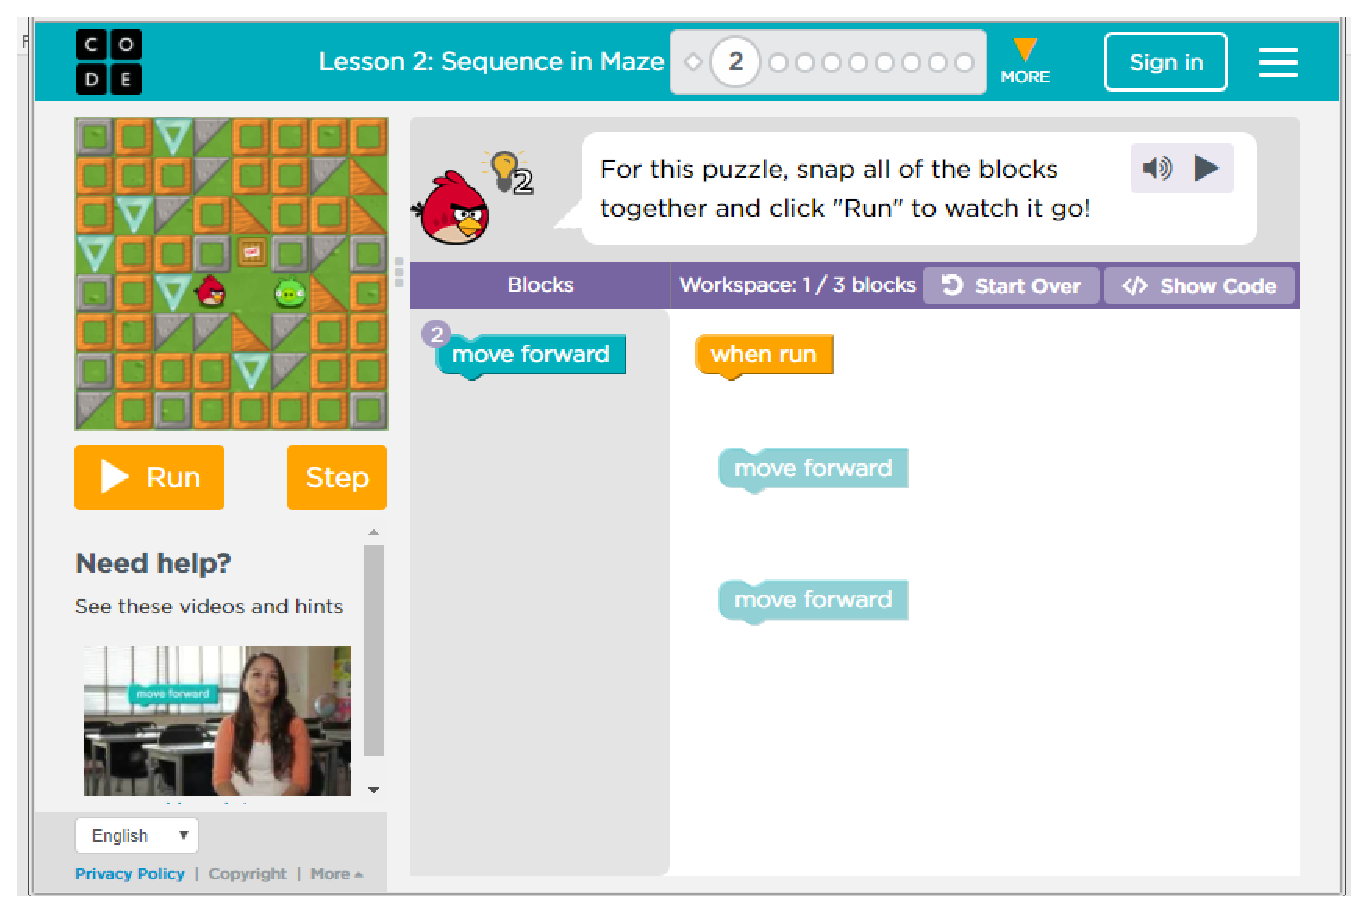
\includegraphics[width=0.6\textwidth]{images/captura_code.eps}
\caption{Code.org}
\label{fig:1}
\end{center}
\end{figure}

En su web se encuentran una serie de cursos y actividades destinados a los alumnos que quieran aprender, organizados por temas y edades. Los profesores, a su vez, pueden aprender a crear talleres para enseñar a sus alumnos en la propia plataforma.

Como se explica en puntos anteriores, fue la plataforma elegida para desarrollar el Trabajo de Fin de Grado, debido a su amplia variedad de cursos a la hora de fomentar el aprendizaje del pensamiento computacional. Su página está destinada a que profesores
enseñen a sus alumnos a través de actividades, mientras que las otras plataformas están enfocadas a aprender de manera autodidacta.

%++++++++++++++++++++++++++++++++++++++++++++++++++++++++++++++++++++++++++++++

\subsection{Codecademy}
\label{2:sec:3}

Codecademy es una empresa enfocada principalmente a la educación y, al igual que Code.org, es una de las plataformas online más relevantes dentro del ámbito de la enseñanza de la programación en la red. Ofrece múltiples cursos gratuitos, de manera que cualquier
persona pueda aprender a programar en diversos lenguajes de programación.

\begin{figure}[!th]
\begin{center}

\includegraphics[width=0.3\textwidth]{images/captura_codecademy.eps}
\caption{Codecademy}
\label{fig:2}
\end{center}
\end{figure}

Los cursos incluidos en la plataforma están estructurados de manera sencilla por temas (sintaxis, funciones, etc.). En caso de que el usuario tenga alguna duda dentro de cada tema, se disponen numerosas clases para dominar los diferentes apartados.

%++++++++++++++++++++++++++++++++++++++++++++++++++++++++++++++++++++++++++++++

\subsection{Programamos}
\label{2:sec:4}

Otra asociación sin ánimo de lucro se llama Programamos, con el objetivo de desarrollar el pensamiento computacional de personas de diferentes edades (desde infantil hasta formación profesional), a través de la programación (en aplicaciones móviles o videojuegos).

\begin{figure}[!th]
\begin{center}
\includegraphics[width=0.3\textwidth]{images/captura_programamos.eps}
\caption{Programamos}
\label{fig:3}
\end{center}
\end{figure}

Algunos de los objetivos que persigue conseguir la plataforma son:

\begin{itemize}
    \item Cambiar el modo de interactuar entre el usuario y la tecnología, para que pase de ser solo consumidor a creador.
    \item Desarrollar capacidades como la creatividad, imaginación, etc.
    \item Permitir al profesorado formarse, de manera que posteriormente pueda enseñar a programar a los alumnos.
\end{itemize}